\documentclass[10pt, fleqn, aspectratio=1610,usenames,dvipsnames]{beamer}
% Preamble for `beamer' slides
% -- Preamble --
\usepackage{xcolor}
\usepackage{colortbl}
\usepackage{multicol}
\usepackage{multirow}
\usepackage{starfont}
\usepackage{hyperref}
\usepackage{etoolbox}	% for TOC spacing fix
\usepackage{parskip}
\usepackage[framemethod=tikz]{mdframed}

% reduce spacing between TOC entries
\makeatletter
\patchcmd{\beamer@sectionintoc}
	{\vskip1.5em}{\vskip0.5em}{}{}
\makeatother

% template settings
\usetheme[progressbar=frametitle]{metropolis}
\setbeamertemplate{frame numbering}[fraction]
\useoutertheme{metropolis}
\useinnertheme{metropolis}
\usefonttheme{metropolis}
\usecolortheme{spruce}

\setbeamercolor{background canvas}{bg=white}
\metroset{block=fill}  % formats `block' display
\hypersetup{
    colorlinks=true,
    linkcolor=blue}
    
% left margin width
\setbeamersize
{text margin left=0.5cm, text margin right=0.5cm}

% alignment 
\defbeamertemplate{description item}{align left}{\insertdescriptionitem\hfill}
\setbeamertemplate{description item}[align left]

% customize default block display
\setbeamertemplate{blocks}[rounded][shadow=true]
\setbeamercolor{block body}{bg=mLightBrown!08}

% -- Macros
\newcommand{\fsc}[1]{\normalfont\scshape{#1}}
\newcommand{\ul}{\rule[0.1in]{\textwidth}{0.2mm}\\ \vspace{-8pt}}
\newcommand*\red{\color{red}}
\newcommand*\dgreen{\color{OliveGreen}}

% -- Variable values for title page
\author{}  % will mess up template if commented out
\date{}     % omit or add your your own date, default is `today'

% -- Override errors
\vfuzz=30pt		% suppress Overfull vbox in Outline
\hypersetup{
	pdfpagelayout=SinglePage,
	pdfauthor={janegca},
	pdfsubject={Hellenistic, Medieval Astrology},
    pdfkeywords={astrology, Greek astrology, Hellenistic astrology, Medieval astrology},
    pdfcreator={TeXworks with pdfLatex, beamer}
}
% -- The Title Slide --
\title{Reception: What will or will not be}
\subtitle{Notes and examples on Reception.}
	\institute{ \large These notes are based primarily on Masha'allah's \textsl{On Reception} trans. Robert Hand, ARHAT, 2nd ed. 1998, and \textsl{Six Astrological Treatises by Masha'allah:The Book of Reception} trans. James Holden, AFA, 2009.
	
\vspace{1em}
	
	Masha'allah tells us that we learn, from reception, \textsl{"Whether something will be or not; when it will be if it should come to pass; when it will become apparent that it will not be if it should not come to pass; what prohibits the matter in case it should not be; and through whom, and from whence it should be if it should come to pass."}[RH p1]}

% -- The Presentation Slides --
\begin{document}
% slides are contained in frames
\begin{frame}
\centering
\begin{minipage}{0.75\textwidth}
\titlepage
\end{minipage}
\end{frame}

% table of contents
\AtBeginSection[]{
	\begin{frame}[t, allowframebreaks]{Outline}
		%\fontsize{7pt}{5pt}\selectfont
		\small
   		\tableofcontents[
   	  		currentsection,
   	  		sectionstyle=show/show,
   	  		subsectionstyle=show/show/hide,
   	  		subsubsectionstyle=show/show/show/hide] 
	\end{frame}
}
% -------------------------------------------------------------------------
\section{Reception Basics}
\subsection{Which Chart Elements are Examined?}
\begin{frame}[t]{Which Chart Elements are Examined?}

The following elements of a chart are examined in judging what will or will not be:
\begin{itemize}
\item[$\bullet$] the 5 planets and two luminaries
\item[$\bullet$] the 12 zodiac signs and their domicile rulers
\item[$\bullet$] the signs of  the Exaltations and Falls of the planets
\item[$\bullet$] the applications and separations of the planets by \Conjunction, \Sextile, \Square, \Trine, or \Opposition\ 
\item[$\bullet$] mutual receptions, return of reception, and "the mutual giving of their disposition"
\end{itemize}
\vspace{0.5cm}

The manner in which a planet commits its \textsl{disposition} helps establish if its significations are effected, prohibited, corrupted, rejected or returned.
\end{frame}

\subsection{What Constitutes Reception?}
\begin{frame}[t]{What Constitutes Reception?}
\small
\textsl{Reception} happens when one planet (A) is in the domicile or exaltation of another planet (B) whom it aspects or conjuncts.

\textbf{Axiom:} {The aspect (or conjunction) from planet \textsl{A} must \textsl{perfect} (become exact)  before that of a third planet (C) intercedes by completing its own aspect or conjunction with planet \textsl{B}. \textbf{This will be true for all reception examples.}}
\vspace{0.1cm}
\begin{columns}[T, onlytextwidth]
\column{0.25\textwidth}
\Mars\ 10 \Aries\ $\Rightarrow$ \Conjunction\ \Saturn\ 15 \Aries
\vspace{1.5cm}
\Mars\ 10 \Capricorn\ $\Rightarrow$ \Square\ \Saturn\ 20 \Aries

\column{0.01\textwidth}
\rule{.1mm}{.4\textheight}

\column{0.75\textwidth}
\Mars\ is applying to the \Conjunction\ of \Saturn\ who is in \Mars's domicile (\Aries), therefore\\
\Mars\ \textsl{receives} \Saturn, but, \\
\Mars\ is not in a domicile (\Capricorn, \Aquarius) or Exaltation (\Libra) of \Saturn, so \\
\Saturn\ \textsl{does not receive} \Mars \\
\vspace{0.1cm}
\ul
\Mars\ is in \Saturn's domicile (\Capricorn) \\
\Saturn\ is in \Mars's domicile (\Aries), therefore, \\
\Mars\ receives \Saturn\ and \Saturn\ receives \Mars\ and \\
there is \textbf{Mutual Reception} [MR] by \textsl{domicile}
\end{columns}
\vspace{0.2cm}
 MR can happen by Exaltation if the two planets are in each other's signs of exaltation. Masha'Allah tells us that if the matter being analyzed has to do with a King, the Exaltation rulers will have more authority over the matter than the domicile rulers.
\end{frame}
\subsection{Applications and Separations}

\begin{frame}[t]{Applications and Separations}
\begin{block}{}
The faster, lighter planet (A) moves to join a slower, heavier planet (B) and in so doing, \textsl{A} commits his disposition to \textsl{B} and the aspect does not leave off until the two planets are separated.
\end{block}

\begin{mdframed}[backgroundcolor=gray!5, rightmargin=2em, leftmargin=2em]
\textbf{Note:} Robert Hand says \textsl{"there is no separating orb"} and so once the two planets are no longer in a partile (exact according to degree) configuration, the matter is done; however, other authors may consider planets to be in aspect as long as they are within the moiety of both. 

The \textsl{moiety} of an aspect between two planets is equal to the addition of half of each planet's orb. For example, the \Sun\ has an orb of 15°, \Saturn\ of 9° so the moiety is 12° (7.5° + 4.5°) or (15° + 9°)/2) so, for some, the pair would not be fully separated until the \Sun\ was 12° past \Saturn.
\end{mdframed}

\begin{block}{}
A planet \textsl{applying to (joining)} another planet indicates \textsl{"what will be"}. 
\end{block}

\begin{block}{}
A planet separating from another planet indicates \textsl{"what has passed away"}.
\end{block}

\end{frame}
\subsection{Committing Disposition}
\begin{frame}[t]{Committing Disposition}
\small
\begin{block}{}
Any planet (A) joining another (B) from \textsl{B}'s domicile or exaltation \textsl{commits its disposition} to \textsl{B}, who, because of reception, will perfect the matter signified by \textsl{A}. A disposition may be \textsl{returned}, possibly in worse condition, if the receiving planet is retrograde, combust, or in its Fall. 
\end{block}

The language used here makes sense in that if \textsl{A} is in a domicile of \textsl{B} he is a guest in \textsl{B}'s home. Astrologically speaking, the ruler of the domicile (B) is responsible for \textsl{settling} or \textsl{disposing} of all matters within his domicile, including those of other planets lodged there. If \textsl{B} is averse (\Semisextile\ or \Quincunx) to its own sign he is blind to the needs of planets in that sign and so he cannot meet their needs unless there is some mitigating condition such as planets in signs that are:

\begin{itemize}
\item \textbf{Like-engirding:}  \Aries\ \Scorpio, \Taurus\  \Libra, \Gemini\ \Virgo, \Sagittarius\ \Pisces,  \Capricorn\ \Aquarius\ (ruled by the same planet)

\item \textbf{Equally Ascending:}  \Aries\ \Pisces, \Taurus\ \Aquarius, \Gemini\ \Capricorn, \Cancer\ \Sagittarius, \Leo\ \Scorpio, \Virgo\ \Libra\ (rise in the same number of hours)

\item \textbf{Seeing-Perceiving:} \Aries\ \Libra, \Taurus\ \Virgo, \Gemini\ \Leo, \Scorpio\ \Pisces, \Sagittarius\ \Aquarius

\item \textbf{Commanding-Obeying:} \Taurus\ \Pisces, \Gemini\ \Aquarius, \Cancer\ \Capricorn, \Leo\ \Sagittarius, \Virgo\ \Scorpio
\end{itemize}
In which cases, \Semisextile's act like a \Conjunction, a \Sextile\ has the power of a \Trine, a \Square's power is doubled, a \Quincunx\ acts like an \Opposition
\end{frame}
% ---------------------------------------------------------------------------------------------------
\begin{frame}[t]{Committing Disposition - An Example}
The nature of the aspect qualifies the nature of the request as a hard one with difficulty, delay, or labour (\Square, \Opposition); an easy one, without labour or difficulty (\Sextile, \Trine), or a familiar, or congenial one, easily done (\Conjunction).

\textbf{Example:}
\begin{columns}[T, onlytextwidth]
\column{0.25\textwidth}
\Sun\ 10 \Aries\ \Square\ \Mars\ 10 \Capricorn

\column{0.01\textwidth}
\rule{.1mm}{.27\textheight}

\column{0.75\textwidth}
the \Sun\ perfects a \Square\  to \Mars, \\
committing his disposition to \Mars, who  \\
receives the \Sun\ in his domicile (\Aries), and so \\
\textsl{accepts} the \Sun's disposition and will perfect it, but \\
due to the \Square\, \\ 
only after some anxiety and errors i.e. not easily
\end{columns}
\end{frame}
% -------------------------------------------------------------------------------------------------
\subsubsection{Committing Disposition - Another Example}
\begin{frame}[t]{Committing Disposition - Another Example}
\textbf{Example:}\footnotemark[1]
\begin{columns}[T, onlytextwidth]
\column{0.25\textwidth}
\Sun\ 1 \Libra\ $\Rightarrow$ \Opposition\ \Saturn\ 25 \Aries

\column{0.01\textwidth}
\rule{.1mm}{.20\textheight}

\column{0.75\textwidth}
the \Sun\ is in \Libra\ (the exaltation of \Saturn) applying to \Opposition\ \Saturn \\
\Saturn\ is in \Aries\ (the exaltation of the \Sun) therefore \\
there is \textbf{Mutual Reception} by \textsl{exaltation}, and \\
the \Sun\ commits his disposition to \Saturn, who accepts it
\end{columns}
\vspace{0.25cm}
According to Masha'Allah, when there is Mutual Reception, \textsl{"there is peace and the matter will be perfected"}; however, if \Saturn\ leaves \Aries\ before the \Opposition\ can perfect, \textsl{"there will be enmities, contrariness, misunderstandings, denials and \Saturn\ will not receive the \Sun"} and so will not take on the \Sun's disposition.

\footnotetext[1]{The examples used by Masha'Allah so far involve planets in their sign of Fall or Detriment which we will see (in later examples), may result in a commitment being returned or corrupted.}
\end{frame}

\subsection{Reception and the Joining of Planets}
\begin{frame}[t]{Reception and the Joining of Planets}
\textbf{Benefics joined to Benefics}

If a benefic (\Venus\ or \Jupiter) joins with and is received by another benefic, the reception increases the good indicated by the planets.

\textbf{Benefics joined to Malefics}

If a benefic (\Venus\ or \Jupiter) joins with and is received by a malefic planet (\Mars\ or \Saturn) then the malefics are at peace and \textsl{"their evil goes away"} unless they are joined by a \Square\ or \Opposition, in which case there will be some labour, and error.

\textbf{Malefics joined to Malefics}

If a malefic (\Mars\ or \Saturn) joins with another malefic with reception, they are made good and their evil and impediment goes away.
\vspace{0.5cm}

\begin{mdframed}[backgroundcolor=gray!5, rightmargin=2em, leftmargin=2em]
\textbf{Note:} the above are generalities based on the essential nature of the planets; there are conditions under which a benefic can act as a malefic and vice versa.
\end{mdframed}

\end{frame}

\section{Horary Rules}
\subsection{Questions in General}
\begin{frame}[t]{Questions in General}

A question must be of great concern or necessity for the querent (the one asking the question); and they should not ask further questions with regard to the matter until the first question has been understood and examined (i.e. no compound questions).

An astrologer should not look to answer his own questions as \textsl{"it does not suit a wise man to look for himself"}. 

To examine the question, draw up a chart for the time the question is asked or verbally put to the astrologer; or, if in the form of a letter, the moment when the astrologer understands what is asked; calculating the Asc, the MC, the places of the 7 planets, and note who disposits each of them and which houses they are in.
\vspace{0.5cm}
\begin{mdframed}[backgroundcolor=gray!5, rightmargin=2em, leftmargin=2em]
\textbf{Note:} James Holden thinks the calculation of the MC implies a quadrant system of houses, most likely Alchabitius, but he acknowledges that Masha'Allah, in later examples, appears to be using a Sign-House system; most likely Equal House\footnote{In Holden's translation of Masha'Allah's \textsl{The Book of Thoughts} he indicates that either the Alchabitius or Equal House system were used.}
\end{mdframed}

\end{frame}
\subsection{Choosing Significators}
\begin{frame}[t]{Choosing Significators}
Masha'Allah's method for choosing which planets will act as significators for the person asking the question (the \textsl{querent}) and the question's subject matter (the \textsl{quesited}), can be reduced to:
\begin{itemize}
\item Does the ruler of the Ascendant (L1) aspect the 1st House?
	\begin{itemize}
		\item Yes? use L1 as the main significator of the querent and the \Moon\ as their partner
		\item No? does L1 aspect another planet that aspects the 1st House or one who does so indirectly by aspecting a 3rd planet that aspects the 1st House?
			\begin{itemize}
				\item Yes? work through these planets and use the \Moon\ as a their partner
				\item No? repeat the same steps using the \Moon\ instead of L1 and if she is suitable, make her the main significator and L1 her partner
			\end{itemize}
	\end{itemize}
\item If neither L1 nor the \Moon\ are usable, see which of the two is the first to leave its sign and judge the effect from that planet's first joining to another planet after entering its new sign, using the other planet (L1 or \Moon) as their partner;\footnote{Normally the \Moon\ is the first to change signs as she moves faster than the other planets.} noting that matters will be slow and inactive until the sign change occurs.
\end{itemize}

\end{frame}
% ------------------------------------------------------------------------------------------
\begin{frame}[t]{Choosing Significators Continued}
\begin{itemize}
\item The main significator of the matter being asked about will be the ruler of the house signifying the matter i.e. Life, ruler of 1st House (L1); Wealth, ruler of 2nd House (L2); Siblings, ruler of the 3rd House (L3); etc.
\item Planets in the 1st House and the house signifying the matter at hand have a bearing on the conditions surrounding the matter BUT they do not determine the outcome of the matter; that depends on the chosen house rulers, their aspects and condition.\footnote{Robert Hand says \textsl{"Rulers of houses in general are more important to outcomes than occupants of houses."}}
	\begin{itemize}
		\item planets in the affected houses, if they are received by their dispositor, \textsl{"indicate the goodness and worthiness of the thing sought"}, if they are not received by their dispositor, then they indicate impediments and the worthlessness of what is sought
	\end{itemize}
\item If the ruler of the Asc or the \Moon\ does not aspect the 1st House it to be considered \textsl{evil and impeded}
\end{itemize}

\end{frame}
\subsection{Perfection and Outcomes}
\begin{frame}[t]{Perfection and Outcomes}
\begin{block}{}
\textsl{Perfection (the performance of a thing) is perhaps known from the planet to which the ruler of the Asc is first joined; from the \Moon; or from the second one that receives the commitment [of the disposition], or namely from whichever one is the last reception [and] there will be the end; or from the ruler of the thing quesited; or from a benefic that is in a good place without reception.} [JH p36]
\end{block}
\textsl{Perfection} can come about in a number of ways ([RH p31, 34])
\small
\begin{itemize}
\item significator of the querent (A) to the significator of the quesited (B), with or without reception, and \textsl{B} does not commit his disposition to a third planet (C)
\item L1 joining a benefic in the house signifying the matter
\item L1 joining a malefic with dignity in the house signifying the matter
\item L1 joining, and received by, an undignified malefic in the house signifying the matter
\item significator of the quesited to L1, with or without reception, or, to planets in the 1st (under the same conditions described for L1 to planets in the house of the matter signified)
\item L1 or the \Moon\ to an angular or strongly dignified benefic, with or without reception; or, a malefic, similarly placed, with reception
\end{itemize}
\end{frame}
% -----------------------------------------
\begin{frame}[t]{Outcomes Continued}

If \textsl{A} is the significator of the querent and receives \textsl{B}, the significator of what is sought; the querent will get what he has been seeking but if \textsl{A} is the significator of what is sought and \textsl{B} is the significator of the querent, then the querent will get what has been asked about without any seeking of it on his part. [JH 38]

Outcomes are better, stronger, more readily done, and stable, and durable if the significator of the quesited receives the significator of the querent. [JH 38]

\begin{block}{}
\textsl{"Reception will not be destroyed in any way whatsoever,...,if the planet which receives has rulership over a matter, and it is the dispositor [of the querent's significator] and the disposition comes to it [the querent's significator applies to it], and if it does not commit disposition to another. Because if it should commit disposition to another planet after its own reception, the reception signifies the accomplishment of the matter, and the commission of its disposition to another planet signifies the end of the matter and to what [state] its final affairs would come."} [RH p32]
\end{block}
So if A applies to its dispositor B, it is received and the matter is accomplished. If B happens to then apply to another planet C, the conditions of that application indicate how the matter will eventually play out.
\end{frame}
% -----------------------------------------
\begin{frame}[t]{Outcomes Continued}

\begin{block}{}
\textsl{"After that, the ruler of the house of the thing [quesited] is looked at to see to what planet it commits its own disposition after its effecting...if it is a benefic, they say the thing will be made better. And if it is a malefic, they say that the thing will be subsequently destroyed."} [JH]p22
\end{block}
If an application by L1 or the \Moon\ shows that the matter will be completed; look to the ruler of the matter being sought (the ruler of the quesited) to see how the matter will play out once it has been effected.

The exception is if the question is about death as there is nothing that can come after it.

If the first joining of the querent's significator is to a malefic and does not involve reception and if the malefic is not the significator of the quesited;  a \textbf{prohibition} is indicated [JH p35].

\end{frame}
\subsection{Timing}
\begin{frame}[t]{Timing  [JH 32-33] [RH 27-29]}
When the joining is by aspect (not conjunction) the number of degrees needed to perfect the aspect gives the number of days.

If it doesn't happen then, it will happen when the two join bodily in a strong place, an angle or a place where the significator of the matter rejoices.

If not then, it will happen when the planet handling the disposition is rising from the \Sun, renewing itself.

If the significators started off Void of Course, needing to enter a new sign before joining with  another planet, then things will go slowly and matters will be prolonged [JH 17, RH 8]

Angles strengthen, hurry, and fortify the matter and, for good or ill, whatever is signified by the ruler of the disposition, it will last. [JH p36]

\end{frame}

\section{Masha'allah's Example Charts}
\subsection{About Life or Death}
\begin{frame}[t]{About Life or Death [JH p18-19,23,27] [RH p10-11,15,19]}
If a person asks whether he will die during the year, look for indications that:\footnote{If L1 is impeded, use the \Moon\ in its place.}
\vspace{0.25cm}
\begin{columns}[T, onlytextwidth]
\column{0.5\textwidth}
\textbf{They will escape death:}\\
\begin{itemize}
\item L1 to a benefic who is not L8 and who does not pass on disposition or return it to another 
\vspace{0.25cm}

\item L1 to a planet that receives him, and if they are ill, they will recover from their illness
\vspace{0.25cm}

\item \Moon\ joined to L8 but L1 strong and unimpeded
\item L8 joined to and received by L1 \textsl{"will not completely destroy"} life
\end{itemize}

\column{0.01\textwidth}
\rule{.1mm}{.45\textheight}

\column{0.5\textwidth}
\textbf{Death wins out:}\\
\begin{itemize}
\item L1 joined to L8 or vice versa (do not consider the \Moon) 
\item L1 joined to a malefic or L8 without reception and the \Moon\ evil and impeded
\item L1 joined to a malefic in the 8th
\item L1 joined, without reception, to a benefic in the 8th who has dignity there
\item L8 joined to a planet in the 1st
\end{itemize}
\end{columns}
\vspace{0.25cm}
To know if the person will fully recover their  'good fortune and health' examine the planet that signifies escape from death; if it aspects the significator's original position in the chart the person will escape all harm.\footnote{Robert Hand fnp11}
\end{frame}
% -----------------------------------------------------------
\begin{frame}[t]{About Life or Death Continued [JH 27-29][RH 19-22]}
\begin{itemize}
\item when L8 joins and is received by L1, L8 cannot completely destroy life but we need to look at L1 and the \Moon\ and if one signifies life and the other death, the significations of L1 are stronger as it has more significance in the matter of Life than the \Moon; however, as they are partners, the \Moon\ will impact the effects of L1 according to the strength or weakness of L1 and the \Moon

\item L8 is inimical to L1 UNLESS they are the same planet as \textsl{"then it will not impedite itself, even if it is also a malefic"} (and the same is true of L1 and L6)
\end{itemize}

\end{frame}
\subsection{Sickness}
\begin{frame}[t]{Sickness [JH]p19-21, [RH]p11-13 }
The question was about a sick person, \textsl{"whether he would be freed from his sickness, or whether he would die"} \\
\vspace{0.25cm}
\begin{columns}[T, onlytextwidth]
\column{0.5\textwidth}
\Mercury\ (L1)  Void of Course in the 8th signifies \textsl{"the strength of pain and the fear of death"} as does \Mars\ (L8) in the 10th aspecting the 1st who signifies \textsl{"the strength of pain and the loss of hope". } \\

\vspace{0.2cm}
\Mercury (L1) is Void of Course, does not aspect the 1st, and is not first to leave his sign. \\

\vspace{0.2cm}
The \Moon\ is also Void of Course but she is \Trine\ the 1st House and she is the first to enter a new sign so she is the stronger significator. \\

\vspace{0.2cm}
The two significators of the querent, both VOC, signified \textsl{"a prolongation of the sickness"} and its severity.\\


\column{0.5\textwidth}
\begin{center}
\vspace{-0.75cm}
{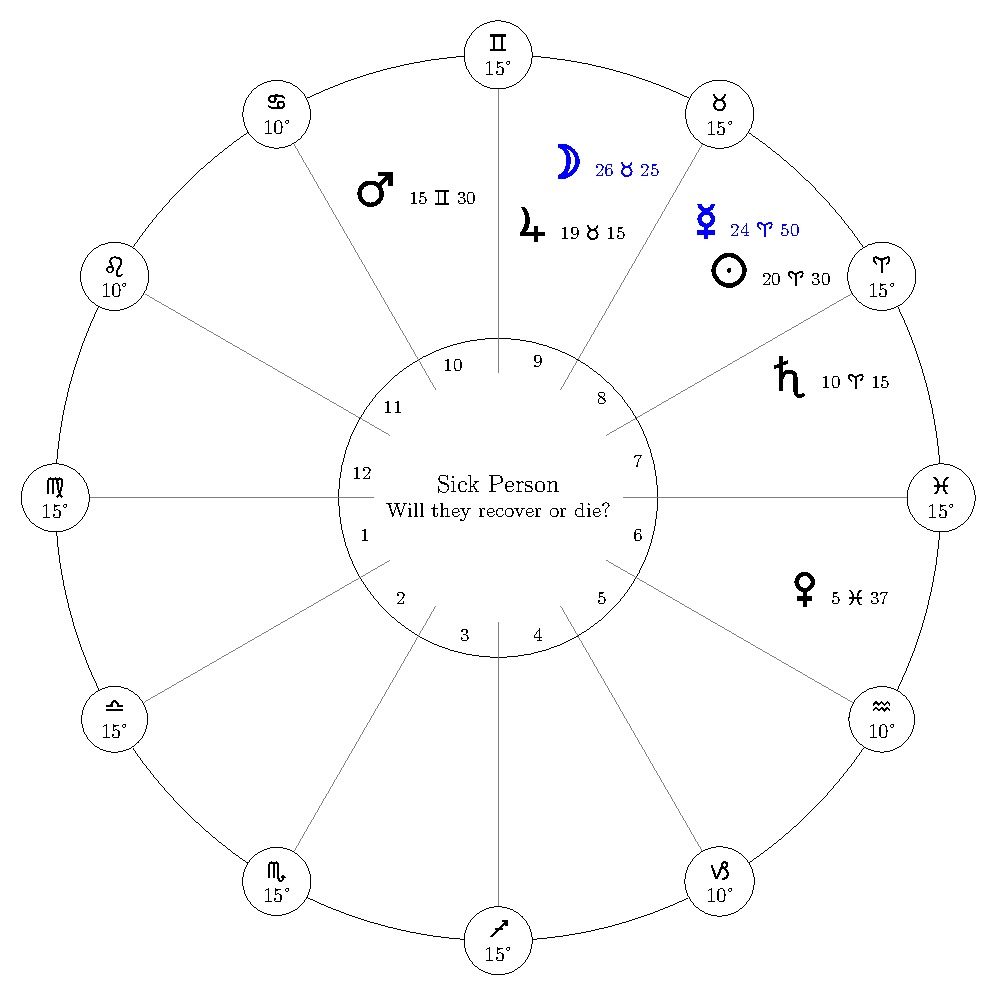
\includegraphics[width=0.9\textwidth]{charts/21-chart-sickness}} \\
\end{center}
\end{columns}

\end{frame}
% ------------------------------------------------------------
\begin{frame}[t]{Sickness Continued}
\begin{columns}[T, onlytextwidth]
\column{0.5\textwidth}
We look at the \Moon, the stronger significator, first. \\
\vspace{0.2cm}
\textbf{\Moon\ in \Taurus\ \Trine\ 1st House} enters \Gemini \\
$\Rightarrow$ \Square\ \Venus\ (in 6th, sickness)  \\
\Venus\ $\Rightarrow$ \Sextile\ \Jupiter, MR by domicile \\

\vspace{0.2cm}
As \Jupiter\ cannot join with any other planet\footnotemark[1], he ends the disposition and becomes the final authority over the matter and so determines the final outcome.

\vspace{0.2cm}
After examining the \Moon\ committing her disposition, Masha'allah looks at \Mercury\ (L1) as sharing in the matter and finds it confirms what the \Moon\ signified.



\column{0.5\textwidth}
\begin{center}
{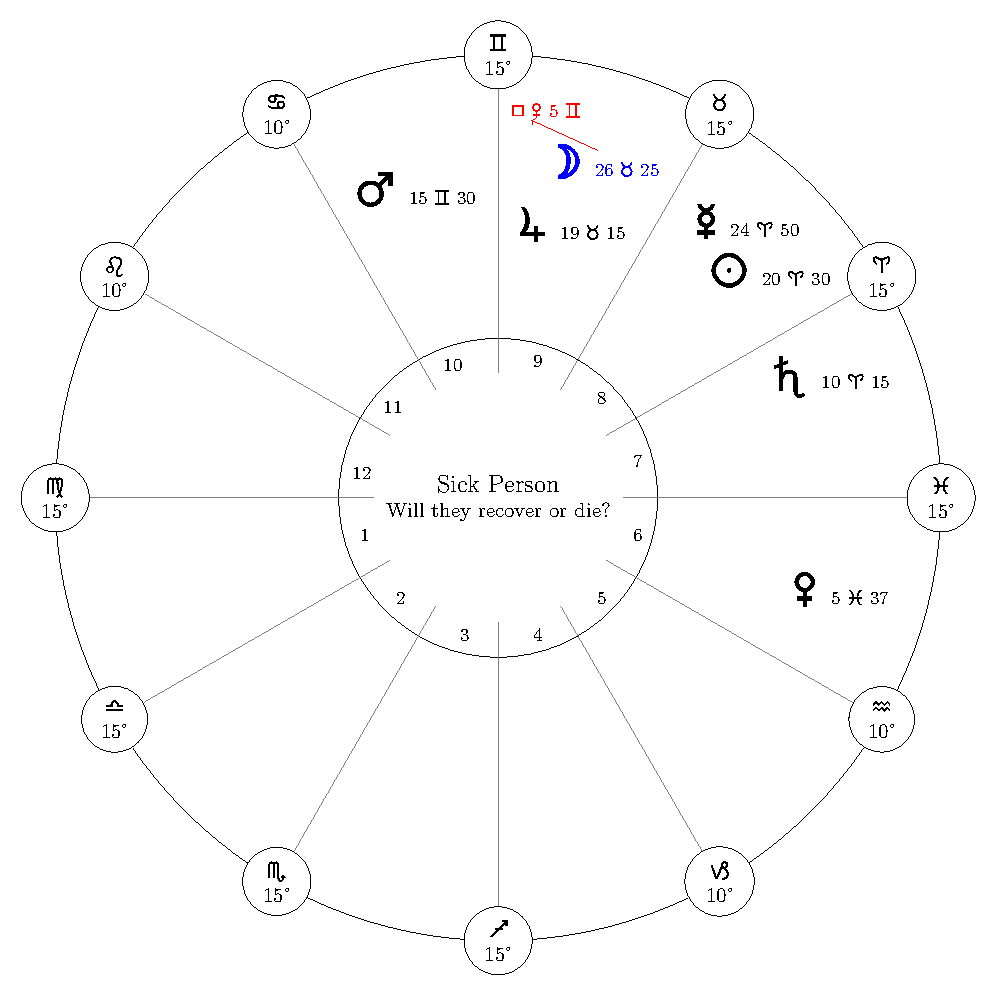
\includegraphics[width=0.9\textwidth]{charts/21a-chart-sickness}} \\
\vspace{-0.2cm}
\end{center}
\end{columns}
\footnotetext[1]{He can only apply to \Saturn\ and he is already separated from him.}
\end{frame}
% ------------------------------------------------------------
\begin{frame}[t]{Sickness Continued}
\begin{columns}[T, onlytextwidth]
\column{0.5\textwidth}

\textbf{\Mercury\ in \Aries\ Void of Course} $\Rightarrow$ \Taurus \\
$\Rightarrow$ \Sextile\ \Venus\ in \Taurus\ accepts his disposition\footnotemark[1] \\
\Venus\ $\Rightarrow$ \Sextile\ \Jupiter\ in \Taurus\, MR by domicile \\
And again, \Jupiter\ is the end of the disposition chain, supporting what the \Moon\ indicated.
\vspace{0.2cm}

\Jupiter, a benefic, as the final arbiter of the disposition promises "health and quiet" and the end of the illness after a prolonged period (due to the VOC's) but we are told that from the time of \Venus\ accepting the \Moon's disposition to her (\Venus's) joining with \Jupiter\ by \Sextile, the person would have gradually strengthened, with the illness leaving him completely once \Venus\ separates from \Jupiter\ by one minute.

\column{0.5\textwidth}
\begin{center}
{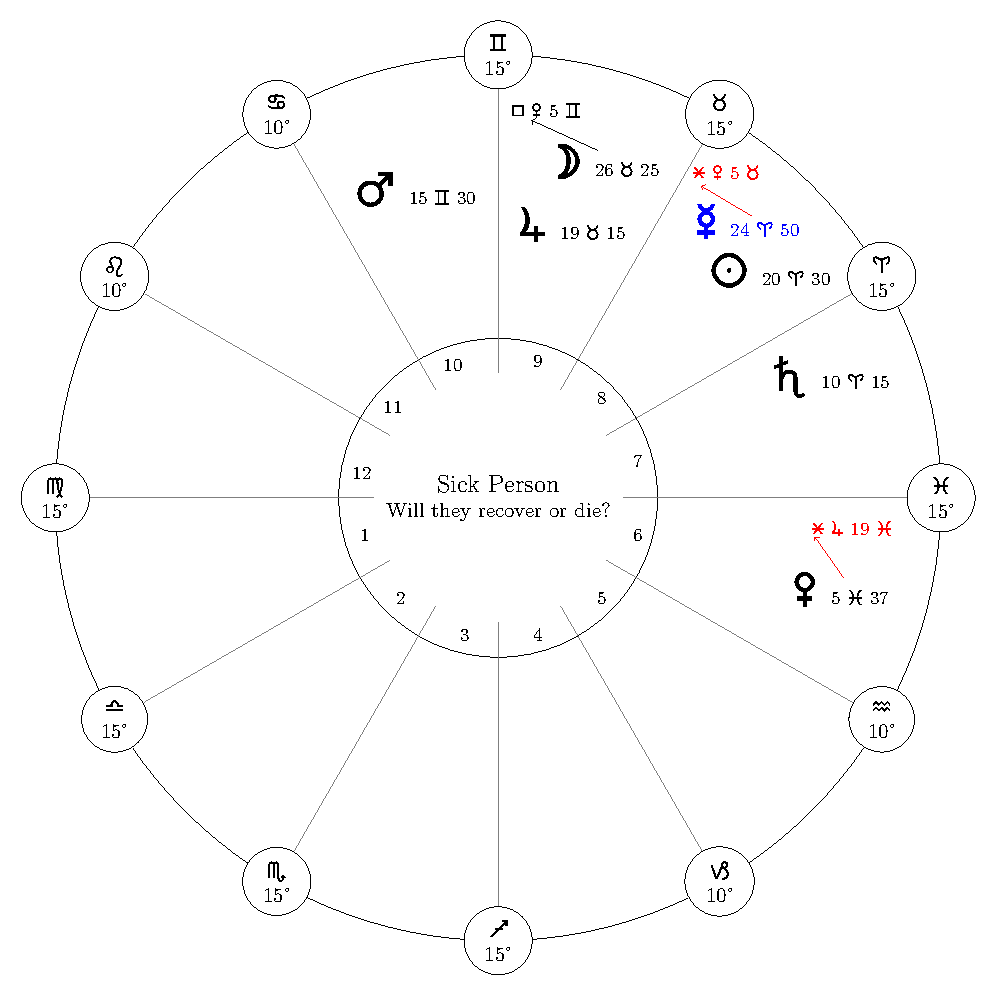
\includegraphics[width=0.9\textwidth]{charts/21b-chart-sickness}} \\
\vspace{-0.2cm}
\end{center}
\end{columns}
\footnotetext[1]{Sahl's mode 14.2, \textsl{Strength of the Planets}, says a planet in dignity can effectively accept a disposition; here it appears to apply to the location of the aspect but it could also apply because \Venus\ has dignity in her place, in \Pisces.}
\end{frame}
% -------------------------------------------------------------------------
\begin{frame}[t]{Sickness (Alternative Scenarios)}
The significator of the matter being asked about (death) is actually \Mars\ as the ruler of the 8th. Masha'allah does list a \Mars\ connection as an alternative scenario, saying such a connection would have meant death for the querent as \Mars's is L8 and does not receive \Venus\ in \Pisces. However, as neither L1 nor the \Moon\ joined to \Mars, the person did not die; although they had a severe illness (\Venus, while not the ruler of the 6th, is in the 6th of sickness). (\textbf{Note:} the \Moon, as the main significator of the querent, is averse to (\Semisextile) \Mars.)\\

\vspace{0.2cm}
He also goes on to warn that had the \Moon\ joined with the \Sun, as he is not L1, he can destroy by combustion if he does not receive the planet, and this also applies to his \Square\ or \Opposition. [JH p23.]\footnotemark[1]

\footnotetext[1]{I've seen this before as a planet being protected from combustion if they are in their own signs; here, the \Moon\ is in her Exaltation but we are told she has to be in the \Sun's signs (\Leo\ or \Aries) to be protected from combustion.}
\end{frame}
\subsection{Example Chart: LIfe Question}
\begin{frame}[t]{Example Chart: Life Question}
\begin{columns}[T, onlytextwidth]
\column{0.5\textwidth}

\column{0.5\textwidth}
\begin{center}
{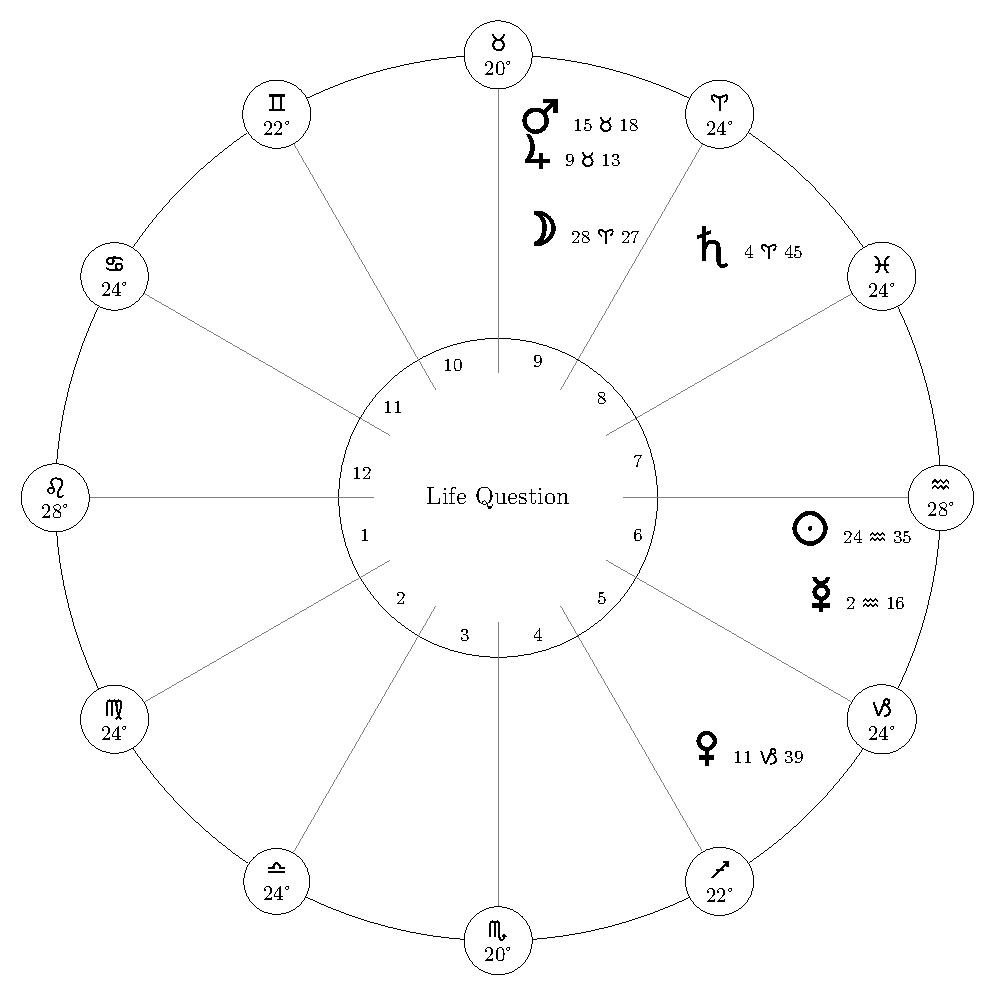
\includegraphics[width=0.9\textwidth]{charts/22-chart-life}}
\end{center}
\end{columns}
\end{frame}

\subsection{Finding Wealth or Not}
\begin{frame}[t]{Finding Wealth or Not [JH 29-31][RH 23-25]}
If the question is about wealth in general, and not specific to some source or person, examine L1 and the \Moon\ to see which is the main significator of the querent and which the sharer and use L2 as the significator of the quesited, wealth.

\begin{block}{}
\textsl{"The connection of the ruler of the Asc or the \Moon\ with the ruler of the thing is the attainment of the thing by itself"}, whether joined to a benefic or malefic, with or without reception, \underline{unless} the significator of the quesited commits its disposition to another planet.\footnotemark[1]
\end{block}

If L2 commits its disposition to:
\begin{itemize}
\item a malefic, with reception, \textsl{"the thing will be perfected"}
\item a benefic, with or without reception, \textsl{"he will find wealth...if the dispositor is in a strong [place] or in the angles"} as angles are useful to the 2nd and hasten things; cadent houses delay things
\end{itemize}

Wealth is also shown if the 2nd holds: a benefic, a dignified malefic, or a malefic without dignity that receives L1.

\footnotetext[1]{Hand says this is true only for the stronger of the two, L1 or \Moon.}
\end{frame}
% -----------------------------------------------
\begin{frame}[t]{Finding Wealth or Not Continued}
If L1 joins with L2 or planets in the 2nd, the querent has been seeking wealth but if L2 joins with L1, the wealth will come about without any seeking on the querent's part and they will receive more than they hoped for.

\textbf{If no L1, \Moon, 2nd House Connections}

If L1 or the \Moon\ do not connect to L2 or a planet in the 2nd, see if one of them connects to a benefic (with or without reception) that is in a strong place or angular; if that benefic does not commit its disposition elsewhere, the querent will find wealth. 

And the same applies if it connects to a malefic with reception but if it is without reception, the matter will be destroyed.

\begin{block}{}
A benefic that commits its disposition to a malefic who does not receive it signifies the matter ruled by the benefic will be harmed when the disposition is complete; with reception, the matter is perfected without harm.
\end{block}

\end{frame}
\subsection{Looking to Borrow}
\begin{frame}[t]{Looking to Borrow}
If a person is looking to borrow from another, L1 and the \Moon\ signify the querent, L2, his wealth while L7 and L8 signify the possible lender and their wealth.

The querent will get what he seeks if:
\begin{itemize}
\item L1 or the \Moon\ are joined to L8 or a planet in the 8th
\item L8 is joined to L1 or a planet in the 1st that is a benefic, a dignified malefic, or a malefic that receives it
\item either  L1 or the \Moon\ is joined to a malefic with reception or a benefic in a strong place
\end{itemize}

But if the person is looking to borrow from the King, use the 11th (Wealth of the King) instead of the 8th.

\end{frame}

\subsection{Inheritance}
\begin{frame}[t]{Inheritance [JH p34] [RH p30]}
\begin{columns}[T, onlytextwidth]
\column{0.5\textwidth}
L1, \Venus\ (16 \Aquarius), was VOC, separating from \Square\  \Jupiter\ (14 \Taurus), L8 (the deceased person's wealth) with reception
\begin{block}{}
\textsl{"Separation by reception is something foul and a horrible thing" [JH 35]}
\end{block}
\Moon\ (28 \Leo) VOC separating from \Opposition\ \Venus\ (16 \Aquarius) \\
\Moon\ first to leave her sign \Leo\ $\Rightarrow$ \Virgo \\
$\Rightarrow$ \Square\ \Mars\ (6 \Virgo), neither planet receives the other, and \\
since \Mars\ is not L8 he signifies prohibition \\
\vspace{0.25cm}
\Venus\ moves from \Aquarius\ to \Pisces \\
$\Rightarrow$ \Square\ \Mars\ (6 \Pisces), neither planet receives the other \\
shows the same as the \Moon; no inheritance

\column{0.5\textwidth}
\begin{center}
{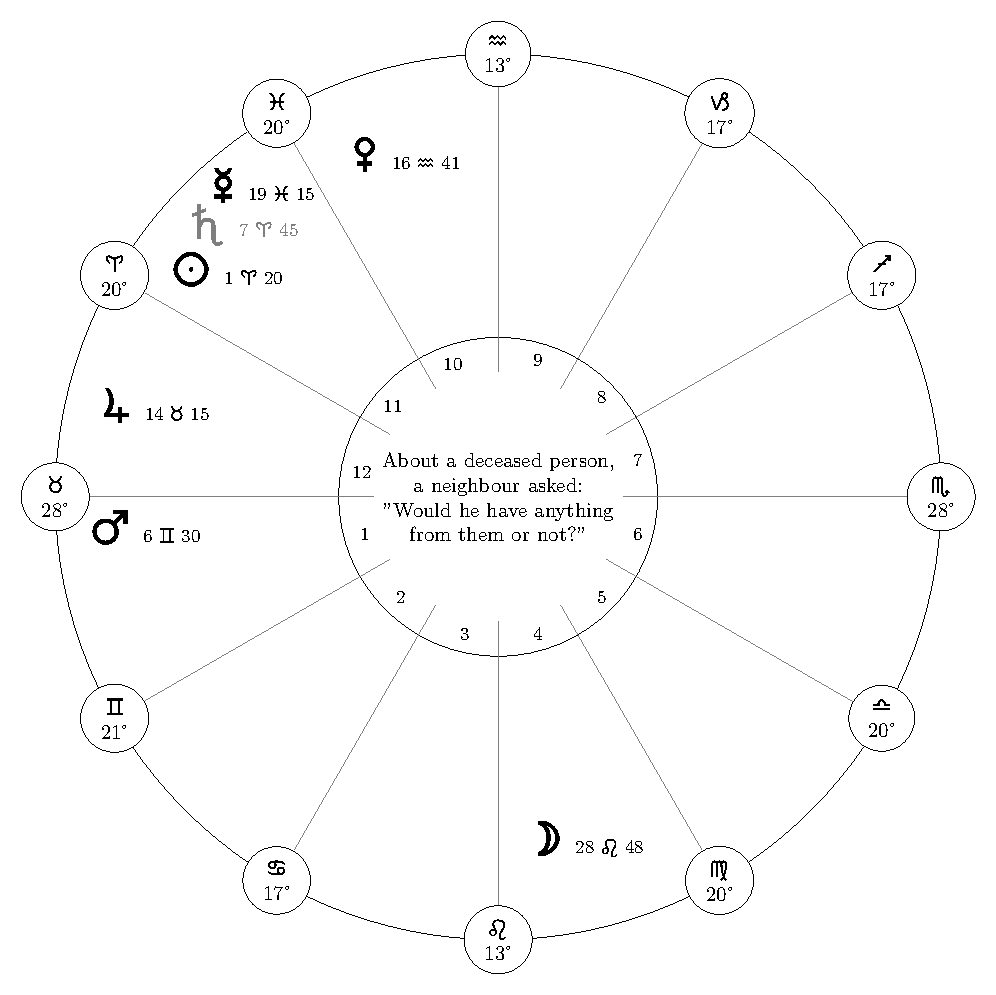
\includegraphics[width=0.9\textwidth]{charts/40-chart-inheritance}} \\
\small
House cusps are not original, Holden shows \Mercury\ at 20 \Pisces; Hand has it at 19 \Pisces\ 15 in the 10th
\end{center}
\end{columns}
\end{frame}

\subsection{Kingdom}
\begin{frame}[t]{Seeking a Kingdom}
\begin{columns}[T, onlytextwidth]
\column{0.5\textwidth}
\Mercury\Retrograde (L1) $\Rightarrow$ \Conjunction\Sun\ $\Rightarrow$ \Sextile\ \Saturn\ (L10) \\
however \\
\Mars\ $\Rightarrow$ \Square\ \Saturn\ (L10) perfects first \\
cutting off the \Sun\ and denying the querent the kingdom \\
\vspace{0.25cm}
And Masha'Allah said the querent would know his hope was lost when \Mars\ perfected its \Square\ to \Saturn \\
\vspace{0.25cm}

Note that the \Moon\ shows the same thing as she first applies to \Mercury, committing her disposition to him and so he hands both his own and her disposition to the the \Sun. And
while  \Mercury\ receives the \Sun, the \Sun\ is not L10 so the matter at hand is not perfected. \\


\column{0.5\textwidth}
\begin{center}
{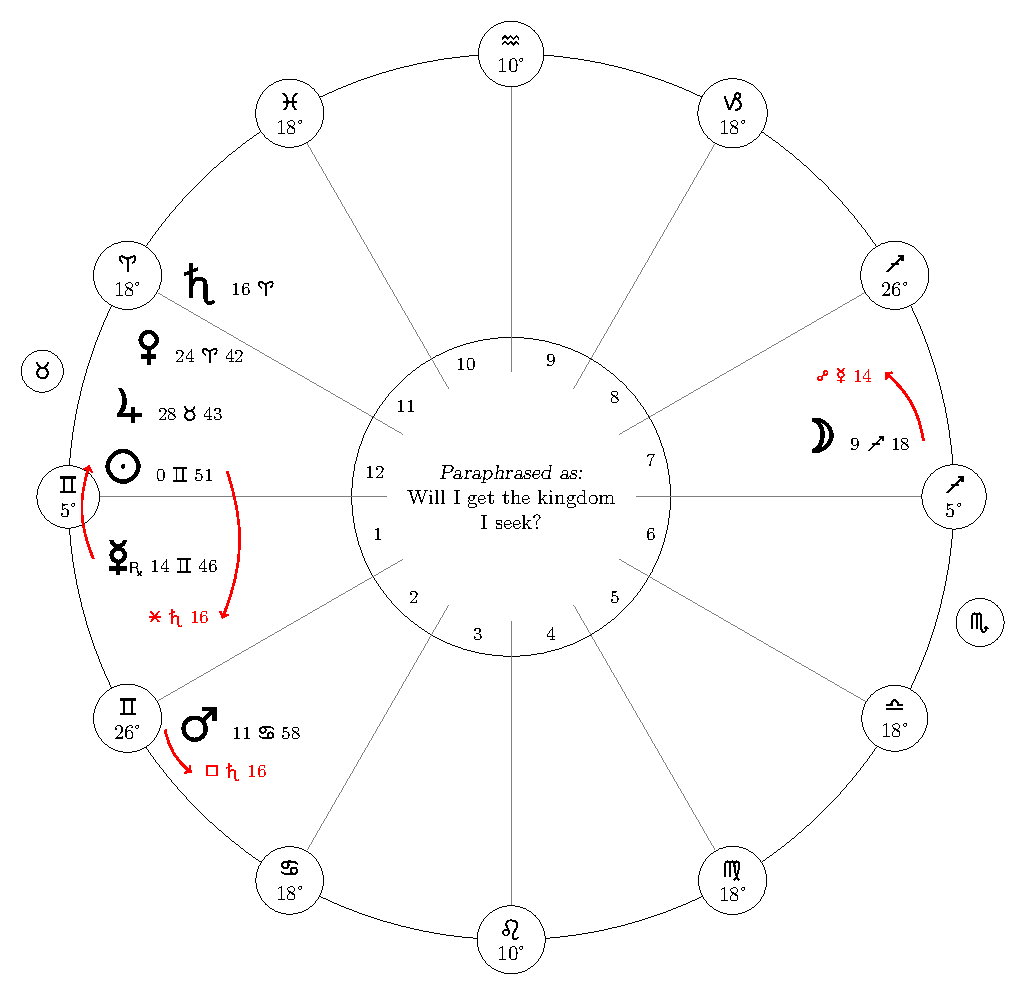
\includegraphics[width=0.9\textwidth]{charts/50-chart-kingdom}} \\
\end{center}
\end{columns}
\end{frame}
% -------------------------------------------------------------------
\begin{frame}[t]{Another Question on a Kingdom}
\begin{columns}[T, onlytextwidth]
\column{0.5\textwidth}
\Moon\ 4 \Libra\ (L1) $\Rightarrow$ \Opposition\ \Saturn\ 11 \Aries\ in the 10th \textsl{"completes"} the matter as \Saturn\ receives the \Moon\ in his exaltation. \\
\vspace{0.5cm}
The man had little joy from his advancement; however, because \Saturn\ was in a place where he had no dignity, being in his Fall and furthermore, in a pitted degree and because it hated its own place it gave something hateful but it made what it gave fixed, strong, and stable because it was in an angle.
 
\column{0.5\textwidth}
\begin{center}
{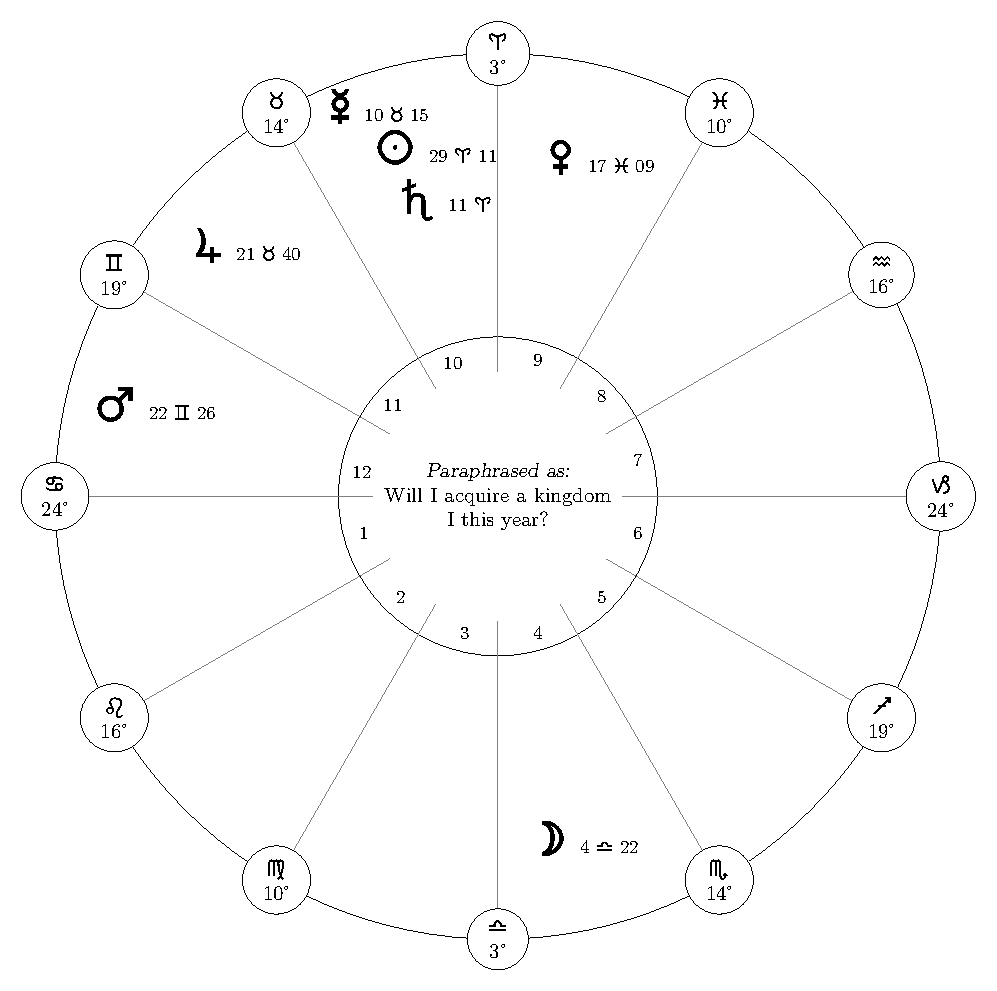
\includegraphics[width=0.9\textwidth]{charts/50-chart-kingdom-1}} \\
\end{center}
\end{columns}
\end{frame}
\input{51-another-kingdom}
\subsection{Will I get the dukedom promised by the King?}
\begin{frame}[t]{Will I get the dukedom promised by the King?}
\begin{columns}[T, onlytextwidth]
\column{0.5\textwidth}
\Jupiter\ is L1, direct, in the 10th (most elevated planet) \\
\hspace{1em}\Sun\ \& \Venus\ $\Rightarrow$ \Square\ from \Sagittarius\ on 1st (received) \\
\hspace{1em}aspects both his domiciles \Sagittarius\ (1st) and \Pisces\ (4th) \\
\hspace{1em}aspects the 7th (connections to all 4 angles) \\
\hspace{1em}signifying he will get his dukedom\\
\vspace{0.5em}
\Mercury\ is L7, retro, a rebel opponent in the matter \\
\hspace{1em}cadent in the 12th \\
\hspace{1em}$\Rightarrow$ \Opposition\ \Saturn\ retro, cadent in 6th\footnotemark[1] (no reception) \\
\hspace{1em}dispositor, \Venus, is combust, worsening matters \\
\hspace{1em}indicates destruction for the opponent \\
\vspace{0.5em}
\Mercury\ retro, by transit, $\Rightarrow$ \Sextile\ \Jupiter\ with reception indicates the rebel opponent will end by seeking "peace and accommodation" from the querent

\column{0.5\textwidth}
\begin{center}
{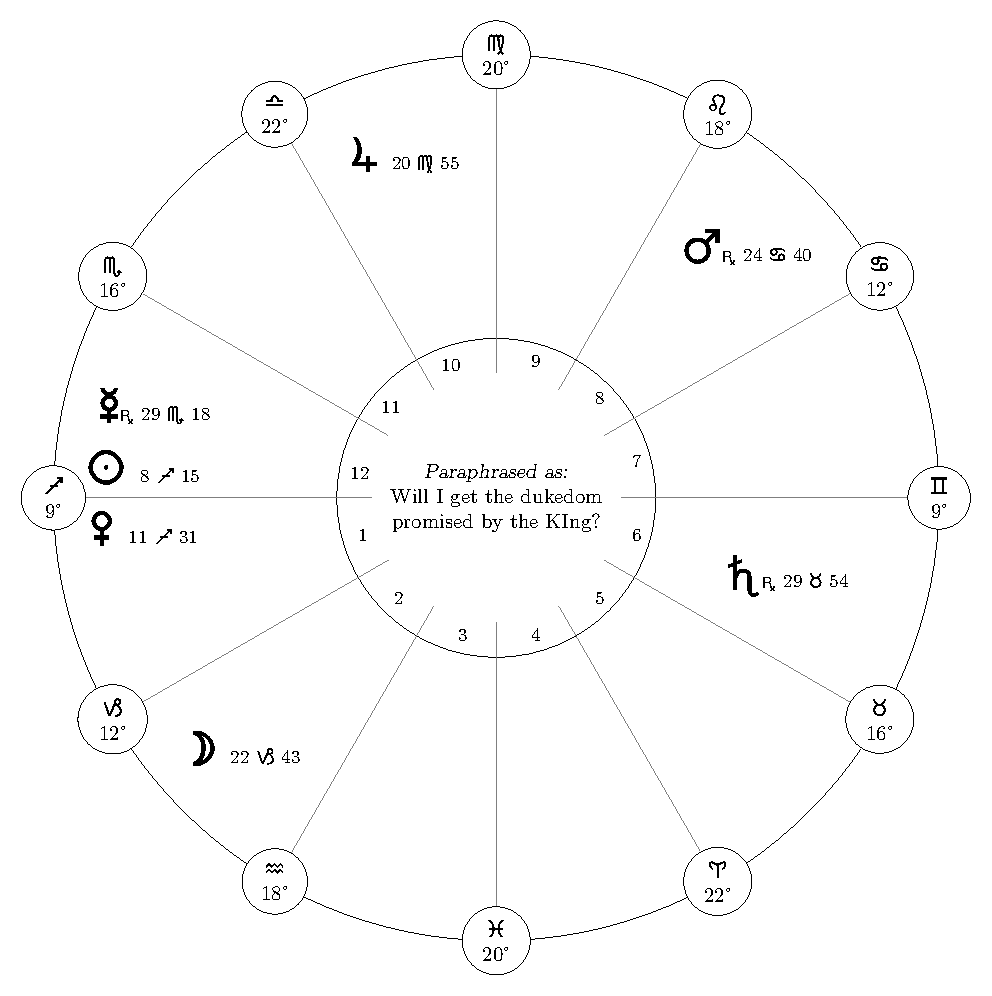
\includegraphics[width=0.9\textwidth]{charts/52-chart-dukedom}} \\
\scriptsize
The MC was not given, only the Asc degree. The other cusps are in the text Holden used but are not original to Masha'Allah.
\end{center}
\end{columns}
\footnotetext[1]{Hand notes this can only be true by Primary Direction.}

\end{frame}
% --------------------------------------------------------------
\begin{frame}[t]{Dukedom Chart as Battle Chart}
Masha'allah goes further into the chart, reading it as a 'battle' or 'war' chart; he begins with the \Moon, using its separating to identify the querent and its application to identify the rebel lord. \\
\vspace{0.25cm}
\Jupiter\ in \Virgo\ \Trine\ (not rec'd) $\Leftarrow$ \Moon\ in \Capricorn\ $\Rightarrow$ \Opposition\ \Mars\ in \Cancer\ (mixed reception) \\
\hspace{1em}\Moon\ is significator of the opponent  in the 2nd (support for querent) \\
\hspace{1em}\Mars\ retro, in 8th, in his Fall; indicating the opponents penury (8th is 2nd from 7th) \\
\hspace{1em} Masha'allah says this indicates the rebel lord could not pay his army \\
\hspace{1em} so the querent bought them off; ending the battle \\
\vspace{0.25cm}
But, as \Mars\ is the dispositor of \Mercury\ (L7), and it is in a strong reception with the \Moon, the rebel lord will not lose everything and, as already noted, \Mercury's \Sextile\ to \Jupiter\ indicates a peaceful conclusion for all involved.

This is the last of Masha'allah's examples.

\end{frame}

\end{document}